\documentclass[11pt]{article}
\usepackage[utf8]{inputenc}
\usepackage[T1]{fontenc}
\usepackage{lmodern}
\usepackage[margin=1in]{geometry}
\usepackage{graphicx}
\usepackage{amsmath}
\usepackage{amssymb}
\usepackage{booktabs}
\usepackage{array}
\usepackage{enumitem}
\usepackage{tcolorbox}
\usepackage{titlesec}
\usepackage{placeins}
\usepackage{fancyhdr}
\usepackage{microtype}
\usepackage{tikz}
\usepackage[round,authoryear]{natbib}
\usepackage[colorlinks=true,linkcolor=paperblue,citecolor=paperblue,urlcolor=paperblue]{hyperref}
\tcbuselibrary{skins}
\usetikzlibrary{arrows.meta,positioning}

% ============================================================
%  EIF Final Culmination: portfolio, reflection and story of my work
%  Build with:  pdflatex eif-final-culmination.tex && bibtex eif-final-culmination
%               && pdflatex eif-final-culmination.tex && pdflatex eif-final-culmination.tex
%  Figures are reused from the other folders of this repository
%  (../whitepaper, ../synthetic-data-generator, ../results-and-discussion),
%  so build with the repository layout intact.
% ============================================================

% ---- colours shared with the whitepaper and the Deliverable 3 slides ----
\definecolor{paperblue}{RGB}{59,103,190}
\definecolor{titlebox}{RGB}{248,247,253}
\definecolor{good}{RGB}{30,132,73}
\definecolor{bad}{RGB}{192,57,43}
\definecolor{ink}{RGB}{35,40,52}
\definecolor{softgray}{RGB}{110,116,128}

% ---- headings ----
\titleformat{\section}{\normalfont\sffamily\bfseries\large\color{paperblue}}{\thesection}{0.6em}{}
\titleformat{\subsection}{\normalfont\sffamily\bfseries}{\thesubsection}{0.6em}{}
\titlespacing*{\section}{0pt}{1.4em}{0.7em}
\titlespacing*{\subsection}{0pt}{1.1em}{0.5em}
\renewcommand{\bibsection}{\section*{Sources}}
\setlength{\bibsep}{3pt}
\setlength{\emergencystretch}{2em}
\setlength{\parindent}{0pt}
\setlength{\parskip}{5pt}

% ---- float placement ----
\renewcommand{\topfraction}{0.9}
\renewcommand{\textfraction}{0.07}
\renewcommand{\floatpagefraction}{0.7}

% ---- footer: the synthetic-data notice is on every page ----
\pagestyle{fancy}
\fancyhf{}
\renewcommand{\headrulewidth}{0pt}
\fancyfoot[L]{\color{softgray}\sffamily\scriptsize Batitay \,$\cdot$\, EIF Final Culmination}
\fancyfoot[C]{\color{bad}\sffamily\bfseries\scriptsize SYNTHETIC DATA: not real students}
\fancyfoot[R]{\color{softgray}\sffamily\scriptsize\thepage}
\fancypagestyle{plain}{\fancyhf{}\renewcommand{\headrulewidth}{0pt}
  \fancyfoot[L]{\color{softgray}\sffamily\scriptsize Batitay \,$\cdot$\, EIF Final Culmination}
  \fancyfoot[C]{\color{bad}\sffamily\bfseries\scriptsize SYNTHETIC DATA: not real students}
  \fancyfoot[R]{\color{softgray}\sffamily\scriptsize\thepage}}

% ---- small helpers ----
\newcommand{\key}[1]{\textcolor{paperblue}{\textbf{#1}}}
\newcommand{\ptag}[1]{\texttt{\small #1}}
\newcommand{\pfield}[1]{\par\vspace{3pt}\noindent{\sffamily\bfseries\color{paperblue}#1}\par\nopagebreak\vspace{-2pt}}
\newcommand{\repo}{https://github.com/machew-b/Student-Retention-Synthetic-Data-Generator}
\newcommand{\gh}[2]{\href{\repo/#1}{#2}}

% A deliverable header bar
\newtcolorbox{deliverable}[1]{enhanced,colback=titlebox,colframe=paperblue!60,boxrule=0.6pt,arc=2mm,
  left=3mm,right=3mm,top=1.5mm,bottom=1.5mm,fonttitle=\sffamily\bfseries,coltitle=white,colbacktitle=paperblue,
  title={#1},attach boxed title to top left={yshift=-2mm,xshift=3mm},boxed title style={arc=1.5mm,boxrule=0pt}}

% Four-quadrant boxes
\newtcolorbox{qbox}[3]{height=#3,valign=top,colback=white,colframe=#1,boxrule=0.8pt,arc=2mm,left=2.5mm,right=2.5mm,top=1.5mm,bottom=1.5mm,
  title={#2},fonttitle=\sffamily\bfseries\small,coltitle=white,colbacktitle=#1,
  before upper={\footnotesize\setlength{\parskip}{2pt}}}

\hypersetup{pdftitle={EIF Final Culmination: The Story of My Student Retention Synthetic Dataset Project},pdfauthor={Matthew C. Batitay},pdfsubject={Eskwelabs Innovation Fellowship, Data Innovation Track},pdfkeywords={portfolio, reflection, synthetic data, student retention, Eskwelabs Innovation Fellowship}}

\begin{document}

% ============================================================ title box
\begin{tcolorbox}[colback=titlebox,colframe=titlebox,arc=4mm,boxrule=0pt,left=10mm,right=10mm,top=6mm,bottom=6mm]
\begin{center}
{\sffamily\bfseries\LARGE EIF Final Culmination:\\[3pt] The Story of My Student Retention\\[3pt] Synthetic Dataset Project}\\[10pt]
{\large Matthew C. Batitay}\\[2pt]
{\itshape Eskwelabs Innovation Fellowship, Data Innovation Track}\\[2pt]
{\small November 2026}
\end{center}
\vspace{6pt}

\noindent\textbf{Projects $\to$ Portfolio $\to$ Story.} This document gathers my fellowship work into one place and asks the question the Final Culmination is built around: what did I do, and what does it say about me? My EIF work is a single Synthetic Dataset project delivered in three parts: a whitepaper that specifies a two-layer model of student dropout in Philippine higher education, a generator and a 50,000-student dataset built from that specification, and an analysis of the dataset that grades common analytics methods against a known true effect. Below I say who I am, how the work unfolded, what each deliverable contains and what I did in it, what I learned, and what I would do next. It is a reflection on work that already exists and a map to its files. It is not a new project, and it makes no claim of being perfect.
\end{tcolorbox}

\vspace{4pt}
\begin{tcolorbox}[colback=white,colframe=bad,boxrule=0.8pt,arc=2mm,left=3mm,right=3mm,top=1.5mm,bottom=1.5mm]
\small\textbf{\textcolor{bad}{Everything numerical in this document is synthetic.}} Each figure below describes the behaviour of a generative model calibrated to cited \emph{aggregate} statistics. None of it measures any real Philippine student or institution, and no number here should be reported as an empirical finding. The only real numbers are the model inputs tagged \ptag{CALIBRATED} with a citation. Parameters carry one of three tags throughout: \ptag{LOCKED} (fixed by design), \ptag{CALIBRATED} (set to reproduce a cited statistic) or \ptag{ASSUMED} (a stated modelling choice without a citation).
\end{tcolorbox}

\vspace{2pt}
\noindent{\sffamily\bfseries\color{paperblue}How this document is organised.}\quad
\textbf{1}~About me \,$\cdot$\, \textbf{2}~My EIF journey \,$\cdot$\, \textbf{3}~Project portfolio \,$\cdot$\, \textbf{4}~Reflection \,$\cdot$\, \textbf{5}~What is next

% ============================================================ 1 ABOUT ME
\FloatBarrier
\section{About Me}
\label{sec:about}

I am Matthew C. Batitay, a Fellow in the Eskwelabs Innovation Fellowship (EIF), Data Innovation Track. My work lives on GitHub as \href{https://github.com/machew-b}{\texttt{machew-b}}, and everything described here is in one public repository: \gh{}{Student Retention Synthetic Data Generator}.

In the fellowship I took on a Synthetic Dataset project: model a real-world system, encode its variables and relationships mathematically, and generate data that reproduces realistic correlations, drop-off and edge cases. I chose student retention in Philippine higher education, a setting where published attrition figures exist only in aggregate, and where records show what a student does but not why a student leaves.

\subsection{How I work}
Four habits run through all three deliverables, and each can be checked in the repository rather than taken on my word.
\begin{itemize}[topsep=2pt,itemsep=2pt,parsep=0pt]
\item \key{Write every assumption down.} All 60 generator parameters carry a provenance tag and are logged in a file. Nothing enters the model untagged.
\item \key{Build in a known answer.} I fixed the true effect of the support programme by design, so any analysis can be scored against the truth rather than only judged plausible.
\item \key{Separate what matched by construction from what was independently checked.} Fitting to a target shows only that a loop converged. I keep that apart from checks that have independent content.
\item \key{Say what the work is not.} The dataset ships with a usage notice, every output carries a synthetic-data banner, and the deck has a slide titled ``what these results are not''.
\end{itemize}

\subsection{Skills snapshot}
\begin{center}
\small
\renewcommand{\arraystretch}{1.2}
\begin{tabular}{@{}>{\raggedright\arraybackslash}p{0.27\textwidth}>{\raggedright\arraybackslash}p{0.43\textwidth}>{\raggedright\arraybackslash}p{0.21\textwidth}@{}}
\toprule
\textbf{Area} & \textbf{What I did with it} & \textbf{Where to see it}\\
\midrule
Statistical modelling and simulation & Latent-variable panel model, discrete-time hazard, nested-bisection calibration with common random numbers & Whitepaper; generator\\
Causal inference & Confounded assignment, Mantel--Haenszel, cluster-robust Poisson, inverse-probability weighting, adjustment-set ladder, DAG & Analytics notebook, Sec.~8\\
Predictive modelling and evaluation & Student-grouped cross-validation, logistic hazard, boosted trees, leakage guard, performance ceilings & Analytics notebook, Sec.~6\\
Python data stack & numpy, pandas, SciPy, statsmodels, scikit-learn, matplotlib & Both notebooks\\
Reproducibility & Seeded independent random streams, SHA-256 fingerprints of every table, pinned requirements, hash-parity tests & Generator; analytics Sec.~3\\
Research and sourcing & Traced national and regional attrition figures to their original reports and cohorts & Whitepaper Sec.~10\\
Technical writing and communication & 29-page whitepaper, folder READMEs, 19-page LaTeX slide deck & All three folders\\
Responsible data practice & Synthetic-data notice, no region names in individual-level tables, regional tier kept out of the flagging model & Whitepaper Sec.~13\\
\bottomrule
\end{tabular}
\end{center}

% ============================================================ 2 JOURNEY
\section{My EIF Journey}
\label{sec:journey}

\subsection{The track, the brief and what ``done'' meant}
The Data Innovation Track's Synthetic Dataset project has three deliverables. I met each with one artefact, and the table below also records what the programme's definition of done required and how I answered it.

\begin{center}
\small
\renewcommand{\arraystretch}{1.2}
\begin{tabular}{@{}>{\raggedright\arraybackslash}p{0.07\textwidth}>{\raggedright\arraybackslash}p{0.38\textwidth}>{\raggedright\arraybackslash}p{0.47\textwidth}@{}}
\toprule
 & \textbf{Deliverable asked for} & \textbf{What I delivered}\\
\midrule
D1 & Data model document with 5+ tables and latent and observed relationships & Whitepaper (v17), 8 tables, hidden and recorded layers, 29 pages\\
D2 & Notebook that generates a customisable number of rows across the tables & Generator notebook v1.0.1 and the 50,000-student dataset it produced\\
D3 & Notebook and/or presentation showcasing analytics on the dataset & Analytics notebook (85 cells), executed HTML export and a 19-page slide deck\\
\bottomrule
\end{tabular}
\end{center}

\begin{center}
\small
\renewcommand{\arraystretch}{1.2}
\begin{tabular}{@{}>{\raggedright\arraybackslash}p{0.36\textwidth}>{\raggedright\arraybackslash}p{0.57\textwidth}@{}}
\toprule
\textbf{Definition of done} & \textbf{How I met it}\\
\midrule
Notebook runs end to end from a clean environment & Library versions are pinned in a \texttt{requirements.txt} in each notebook folder. The generator runs in about 30 to 50 seconds at 50,000 students, and the analysis in about 10 to 15 minutes.\\
Every assumption and distribution choice is written down & 60 generator parameters (51 \ptag{ASSUMED}, 6 \ptag{CALIBRATED}, 3 \ptag{LOCKED}) in \texttt{parameter\_log.csv}; the analysis adds its own tagged registry; limitations are logged as open flags OF-1 to OF-12 and DF-1 to DF-9.\\
Data survives a sanity check, with at least two deliberate edge cases & 29 integrity checks plus a correlation test; two engineered edge cases (2,937 and 774 student-terms).\\
A short README states what a user could analyse & The generator README lists five uses, from dropout prediction to estimator-choice exercises.\\
\bottomrule
\end{tabular}
\end{center}

\subsection{The path through the work}
The work did not run in a straight line. The specification came first, the generator exposed where the specification and its implementation disagreed, and the analysis then stress-tested those disagreements instead of hiding them.

\begin{center}
\begin{tikzpicture}[
  box/.style={rounded corners=3pt,draw=paperblue,fill=titlebox,align=center,text width=2.55cm,minimum height=2.3cm,inner sep=3pt,font=\sffamily\scriptsize,text=ink},
  arr/.style={-{Latex[length=2mm]},paperblue,thick}]
\node[box] (a) {\textbf{\normalsize 1}\\[1pt]\textbf{Choose the system}\\Why students leave, and what records miss};
\node[box,right=0.62cm of a] (b) {\textbf{\normalsize 2}\\[1pt]\textbf{Whitepaper v17}\\Eight tables, Eqs.~1--4, tagged parameters, validation plan};
\node[box,right=0.62cm of b] (c) {\textbf{\normalsize 3}\\[1pt]\textbf{Generator v1.0.1}\\50,000-student dataset, 29 checks, scorecard};
\node[box,right=0.62cm of c] (d) {\textbf{\normalsize 4}\\[1pt]\textbf{Analytics}\\85-cell notebook, HTML, 19-page deck, 11 scenarios};
\node[box,right=0.62cm of d,fill=paperblue,text=white,draw=paperblue] (e) {\textbf{\normalsize 5}\\[1pt]\textbf{Final Culmination}\\This portfolio: story, reflection, next steps};
\draw[arr] (a)--(b); \draw[arr] (b)--(c); \draw[arr] (c)--(d); \draw[arr] (d)--(e);
\draw[dashed,softgray,-{Latex[length=2mm]},thick] (c.south) to[out=-90,in=-90,looseness=0.7]
  node[midway,below=1pt,font=\sffamily\scriptsize,text=softgray,align=center]{realised targeting differed from the design (OF-1): documented, then tested in step 4} (d.south);
\end{tikzpicture}
\end{center}
\vspace{10pt}

\subsection{The good, the bad, the old, the new}
\label{sec:gbon}
\begin{minipage}[t]{0.485\textwidth}
\begin{qbox}{good}{The good}{4.6cm}
The analysis notebook carries a verbatim copy of the generator engine and regenerates all eight tables bit for bit. Seven of seven comparable scorecard rows re-derive identically from the CSV files.

Because the true effect is known (30\%), methods can be graded. The naive comparison says support \emph{raises} dropout by 57.7\%, while Mantel--Haenszel gives a 32.2\% reduction (95\% CI 24.3\% to 39.3\%).
\end{qbox}
\end{minipage}\hfill
\begin{minipage}[t]{0.485\textwidth}
\begin{qbox}{bad}{The bad}{4.6cm}
The whitepaper's design targeting (70\% sensitivity, 25\% false flags) is not what the generator realises (about 16\% and 22\%). I did not re-fit the assignment parameters to force a match (OF-1).

The held-out check passes only narrowly: 1.673 against a band of 1.2 to 1.7, with about 60\% of 20 replicate populations inside the band. Inverse-probability weighting swings from $-47\%$ to $+72\%$ across populations.
\end{qbox}
\end{minipage}

\vspace{5pt}
\begin{minipage}[t]{0.485\textwidth}
\begin{qbox}{softgray}{The old}{3.1cm}
The whitepaper's Appendix A reports a \emph{pilot} implementation (Mantel--Haenszel 25.5\%, held-out ratio 1.72, not passed). Generator v1.0.0 kept its frozen calibration constants rounded and left some structural counts untagged.
\end{qbox}
\end{minipage}\hfill
\begin{minipage}[t]{0.485\textwidth}
\begin{qbox}{paperblue}{The new}{3.1cm}
Version 1.0.1 stores the calibration at full precision and tags every number. The released dataset's numbers supersede the pilot's. The analysis adds eleven recalibrated sensitivity scenarios, which answer the question OF-1 left open, and a plain statement of what the results are not.
\end{qbox}
\end{minipage}

% ============================================================ 3 PORTFOLIO
\section{Project Portfolio}
\label{sec:portfolio}

My EIF work is one project with three deliverables. Each is presented the same way: the problem or context, my role and contributions, the output, and the skills it demonstrated. The aim is that a reader who has seen nothing else can tell what I actually did.

\subsection{The project at a glance}
\pfield{Problem / Context}
Philippine tertiary records show what a student does (grades, attendance, financial-account status) but not why a student leaves, and no public dataset links the two at the individual level. National and regional attrition figures exist, but they are aggregates and do not all trace to the same cohort. Retention early-warning systems also tend to base support on the same signals that predict dropout, so the effect of a support programme cannot be read off a naive comparison. Reviews of the dropout-prediction literature describe this as an actionability gap: strong predictive accuracy but little evidence that predictions become interventions that work \citep{dropout2026review}.

\pfield{The idea}
I treated the gap between recorded and true state as the thing to model. A hidden layer (a student's baseline vulnerability $v_i$ and a per-term acute shock) drives both the recorded data and the dropout, and is never exported. Support is assigned from \emph{prior-term} signals, and the true effect is fixed at a risk ratio of exactly 0.70 (\ptag{LOCKED}, a design constant and not an empirical estimate). With $\sigma$ the logistic function, the two mechanisms that matter most are
\begin{align}
\text{risk}_{it} &= \sigma\bigl(\beta_0 + \beta\,k_{it}\bigr), \qquad k_{it} = \mathbb 1(\text{grade}_{i,t-1}<\tau_g) + \mathbb 1(\text{attend}_{i,t-1}<\tau_a) + \text{hold}_{i,t-1},\\
h_{it} &= \sigma\bigl(\gamma_0 + \gamma_1 v_i + \gamma_2\,\text{shock}_{it}\bigr)\times\bigl(1 - 0.30\cdot\text{support}_{it}\bigr),
\end{align}
Here $k_{it}$ counts the prior-term signals that fire. Support is drawn as $\text{Bernoulli}(\text{risk}_{it})$ from term 2 onward, so it depends on observed signals that also predict dropout, and dropout is drawn as $\text{Bernoulli}(h_{it})$ with the true effect built into the second line. Everything downstream is a test of whether an analyst can recover that effect.

% ---------------------------------------------------------------- D1
\subsection{Deliverable 1: The whitepaper (data model)}
\begin{deliverable}{Deliverable 1 \quad Whitepaper: the data model}
\small \emph{A Two-Layer Synthetic Data Generator for Studying Student Retention Early-Warning Systems in Philippine Higher Education}. 29 pages, version 17, in \gh{tree/main/whitepaper}{\texttt{whitepaper/}}
\end{deliverable}

\pfield{Problem / Context}
Deliverable 1 asks for a data model with at least five tables and an explicit relationship between latent and observed variables. The difficulty is specific: published attrition figures disagree, no individual-level mechanism data is public, and a model that cannot be checked against anything is just a story.

\pfield{My role and contributions}
\begin{itemize}[topsep=1pt,itemsep=2pt,parsep=0pt]
\item Designed the eight-table schema (\texttt{Regions}, \texttt{Students} and six student-by-term panel tables) and a five-phase generation pipeline for 50,000 students over up to eight terms (\ptag{LOCKED}).
\item Wrote the generative forms, including the confounded assignment rule and the fixed 30\% effect, so that the model has a built-in answer key.
\item Traced the calibration targets to their sources \citep{cpbrd2026,edcom2025y2,ched2025presentation,pids2024}. I calibrated to the Class-of-2022 tier rates (67.1\% high tier, 45.9\% typical tier, \ptag{CALIBRATED}) and held a separate national figure of 29.4\% out for an independent check.
\item Wrote the validation plan so that calibration-until-convergence is kept distinct from checks with independent content, following the verification-and-validation practice in \citet{law2015}: a held-out check, a confounding check and a recoverability check.
\item Specified two deliberate edge cases (an unflagged high-risk student and a falsely flagged student) and a responsible-use section covering misrepresentation risk and regional framing.
\item Added a field-level schema, integrity rules and a reproducibility policy as Appendix B, which the generator is later checked against.
\end{itemize}

\pfield{Output}
The \gh{blob/main/whitepaper/student-retention-data-generator-model.pdf}{whitepaper PDF}, its \gh{blob/main/whitepaper/student-retention-data-generator-model.tex}{LaTeX source} and bibliography, and two figure scripts. Figure~\ref{fig:pipeline} shows the pipeline.

\begin{figure}[tbp]
\centering
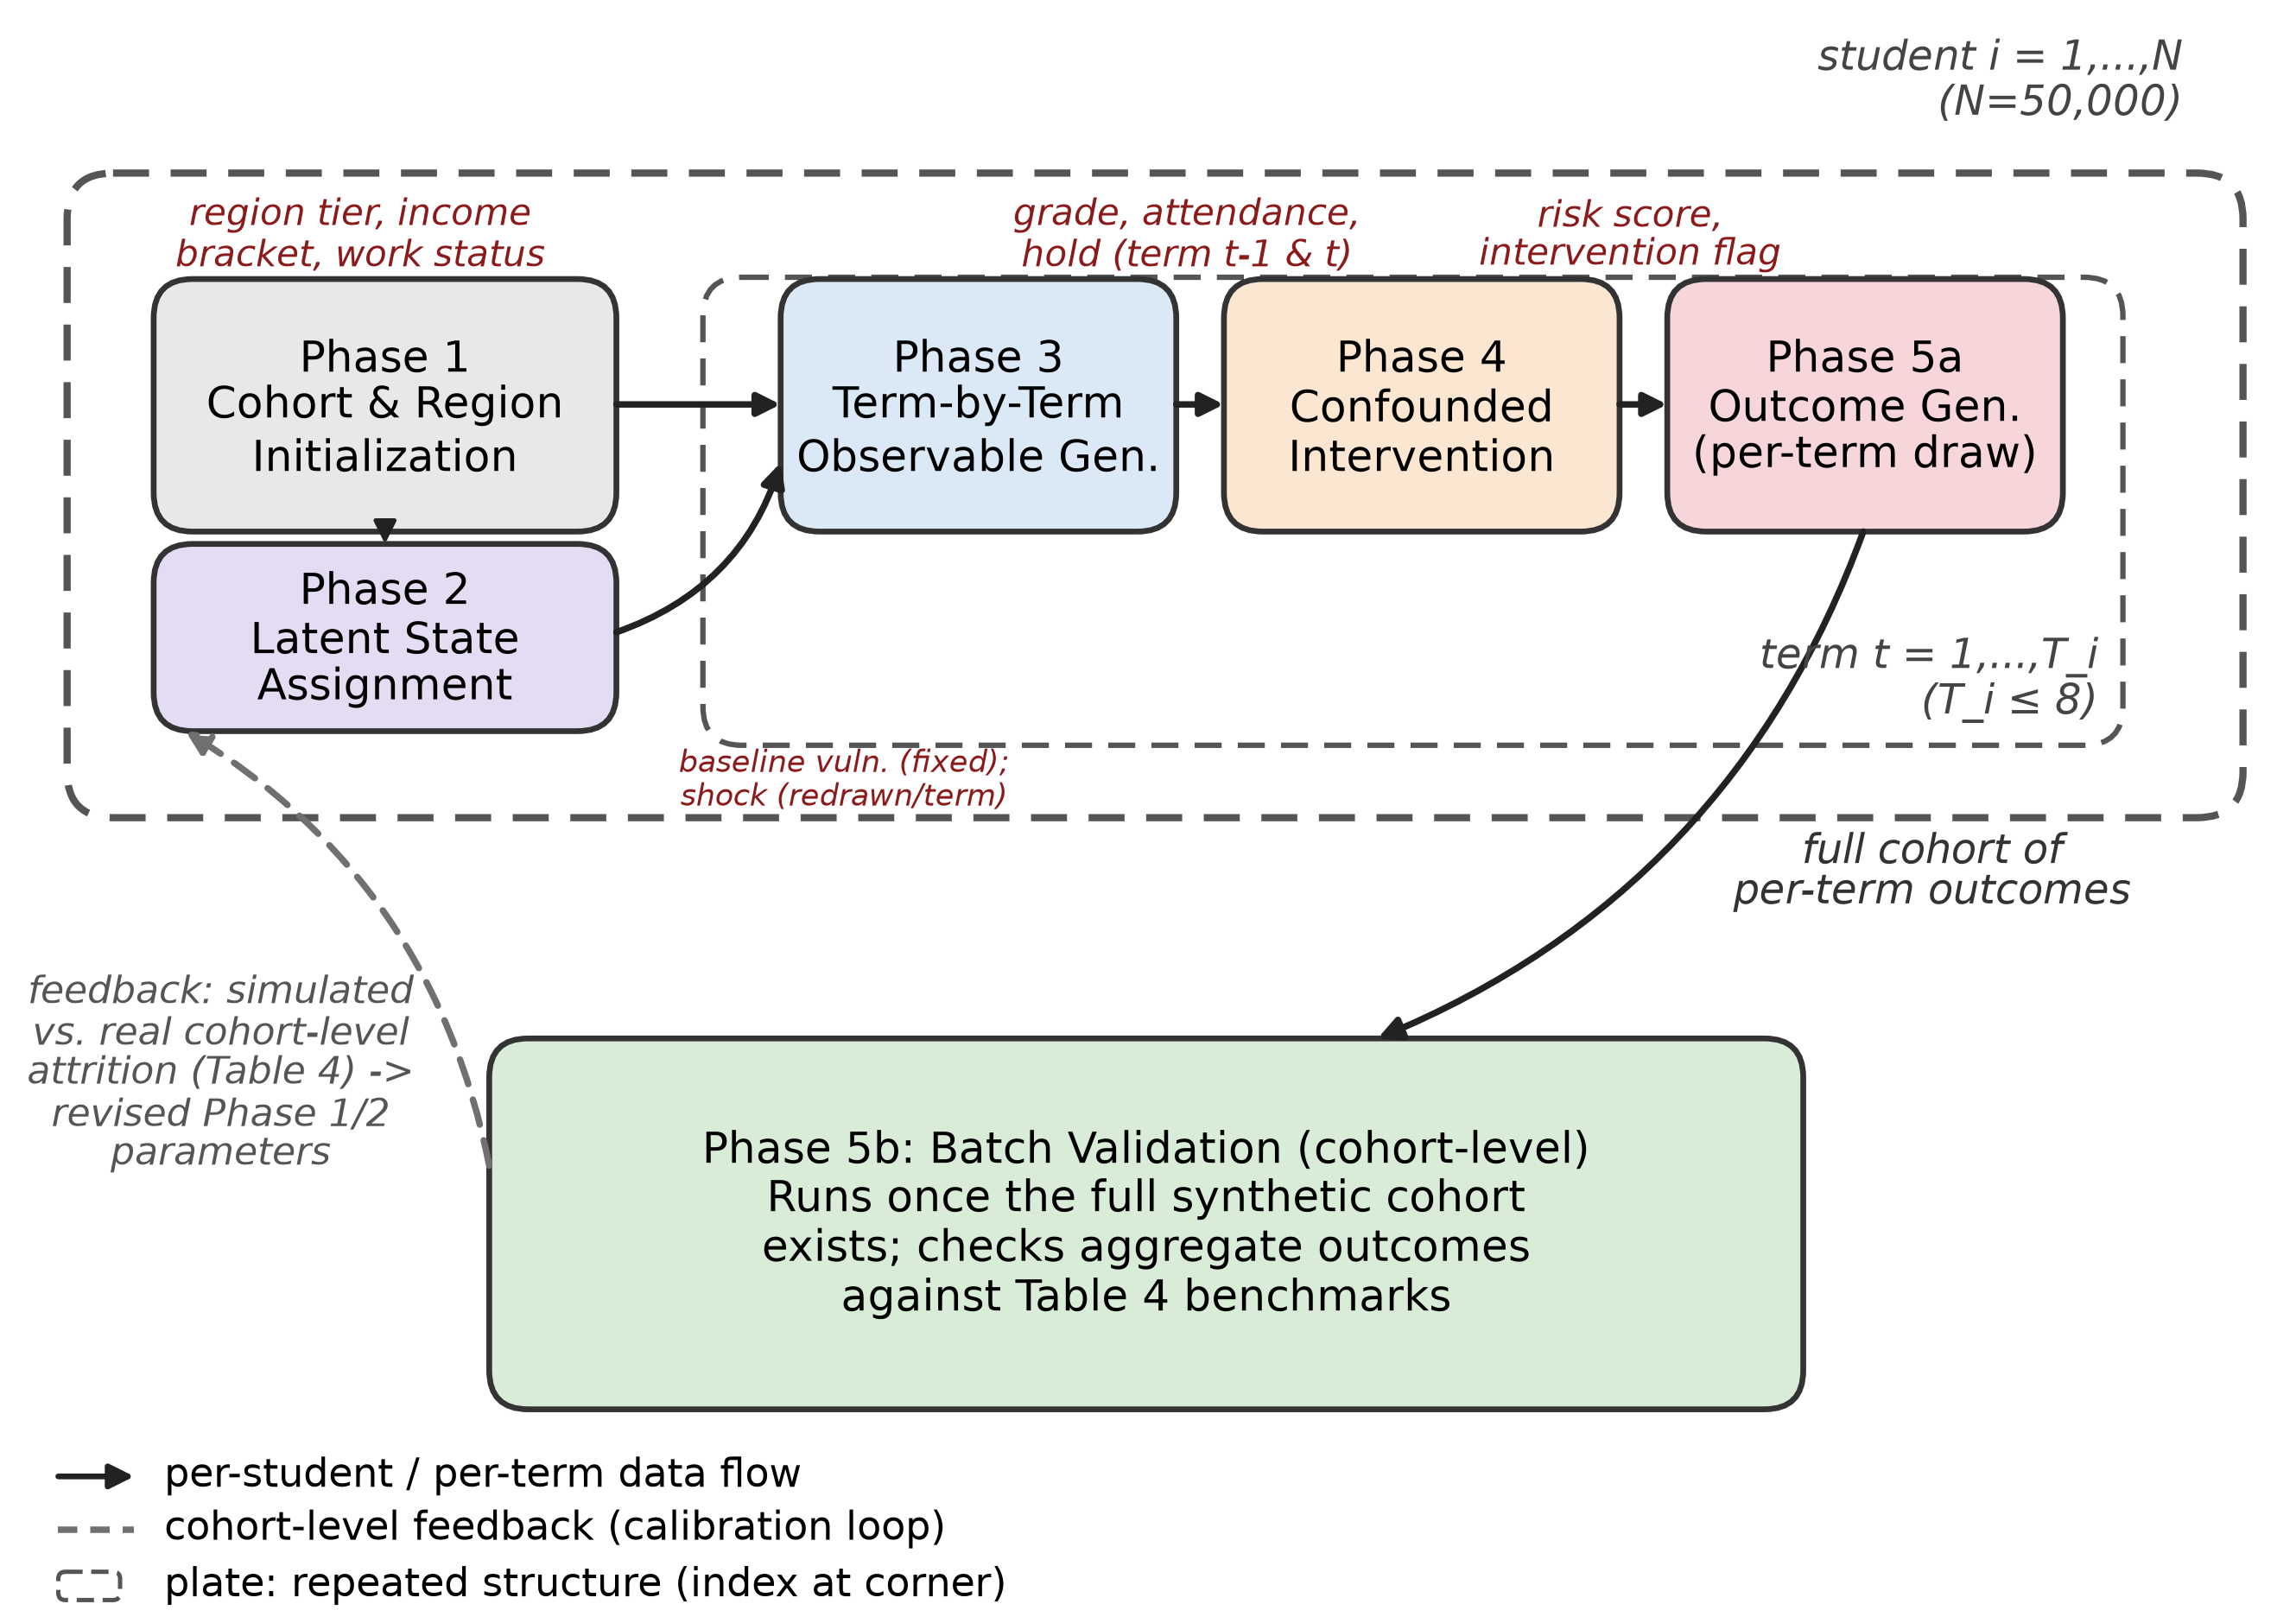
\includegraphics[width=4.0in]{../whitepaper/figures/fig1_pipeline.png}
\caption{The end-to-end pipeline from the whitepaper. Phases 1 to 4 and the per-term outcome draw (5a) repeat for each student and term; batch validation (5b) runs once on the full cohort and feeds back into the calibration (dashed arrow). Whitepaper Figure 1.}
\label{fig:pipeline}
\end{figure}

\pfield{Skills demonstrated}
Data modelling and schema design; latent-variable and hazard modelling; reading and tracing primary sources; designing validation that distinguishes calibration from testing \citep{law2015,gelman2020ros}; technical writing in LaTeX; research ethics for synthetic data.

% ---------------------------------------------------------------- D2
\subsection{Deliverable 2: The generator and the dataset}
\begin{deliverable}{Deliverable 2 \quad Generator v1.0.1 and the dataset}
\small One notebook (36 cells), eight tables, 297,739 rows in each panel table \,$\cdot$\, \gh{tree/main/synthetic-data-generator}{\texttt{synthetic-data-generator/}}
\end{deliverable}

\pfield{Problem / Context}
A specification only counts if it can be run. Deliverable 2 asks for a notebook that generates a customisable number of rows across the tables, and the programme's definition of done also asks for written assumptions, a sanity check and at least two edge cases. The practical problem is that the calibration targets are cohort-level, so the generator has to find its own hazard parameters.

\pfield{My role and contributions}
\begin{itemize}[topsep=1pt,itemsep=2pt,parsep=0pt]
\item Implemented the generator from the whitepaper. A single configuration cell sets the number of students, the master seed, whether to recalibrate and the output folder.
\item Built a parameter registry in which every number is read through one function and carries a tag. The registry is exported as a log: 60 parameters, 51 \ptag{ASSUMED}, 6 \ptag{CALIBRATED}, 3 \ptag{LOCKED}.
\item Drew every random quantity from its own named random stream under one master seed, and used common random numbers so that the calibration loop is stable. A nested bisection fits the tier shift and the hazard intercept to the two tier targets.
\item Wrote 29 integrity checks and a correlation test, a scorecard for every check in the whitepaper's validation table, an audit of the two edge cases, and an assumptions log with open flags OF-1 to OF-12.
\item Shipped version 1.0.1 after finding that v1.0.0 kept its frozen calibration rounded and left some structural counts untagged, so that the default dataset reproduces exactly and no number is untagged.
\item Withheld the hidden state: baseline vulnerability, shocks and the hazard are never exported, and no individual-level table carries a region name.
\end{itemize}

\pfield{Output}
Eight CSV tables (\texttt{Regions} 2 rows, \texttt{Students} 50{,}000, six panel tables of 297{,}739 rows), \texttt{metadata.json} with the SHA-256 of every table, the parameter log, the validation scorecard, a dataset notice and a diagnostics figure (Figure~\ref{fig:diag}). Table~\ref{tab:score} summarises the scorecard.

\begin{table}[htbp]
\caption{Validation scorecard of the released dataset (synthetic; model behaviour, not reality). The first two rows are calibration, not independent validation.}
\label{tab:score}
\centering\small
\renewcommand{\arraystretch}{1.15}
\begin{tabular}{@{}>{\raggedright\arraybackslash}p{0.34\textwidth}>{\raggedright\arraybackslash}p{0.48\textwidth}>{\raggedright\arraybackslash}p{0.12\textwidth}@{}}
\toprule
\textbf{Check} & \textbf{Result} & \textbf{Verdict}\\
\midrule
Tier attrition, high / typical & 67.1\% / 45.9\% (calibrated targets) & Pass\\
Pooled attrition (derived) & 49.1\% & Pass\\
Held-out tier ratio, band 1.2 to 1.7 & 1.673; over 20 populations $1.692 \pm 0.025$, about 60\% in band & Pass (fragile)\\
Confounding present & Naive estimate $-57.7\%$ (CI $-64.6\%$ to $-50.6\%$) excludes the true 30\% & Pass\\
Effect recoverable & Mantel--Haenszel 32.2\% (CI 24.3\% to 39.3\%); Poisson 33.6\% (CI 25.1\% to 41.2\%) & Pass\\
Parameter traceability & 60 parameters, none untagged & Pass\\
Edge cases present & 2,937 and 774 student-terms & Pass\\
\bottomrule
\end{tabular}
\end{table}

\begin{figure}[tbp]
\centering
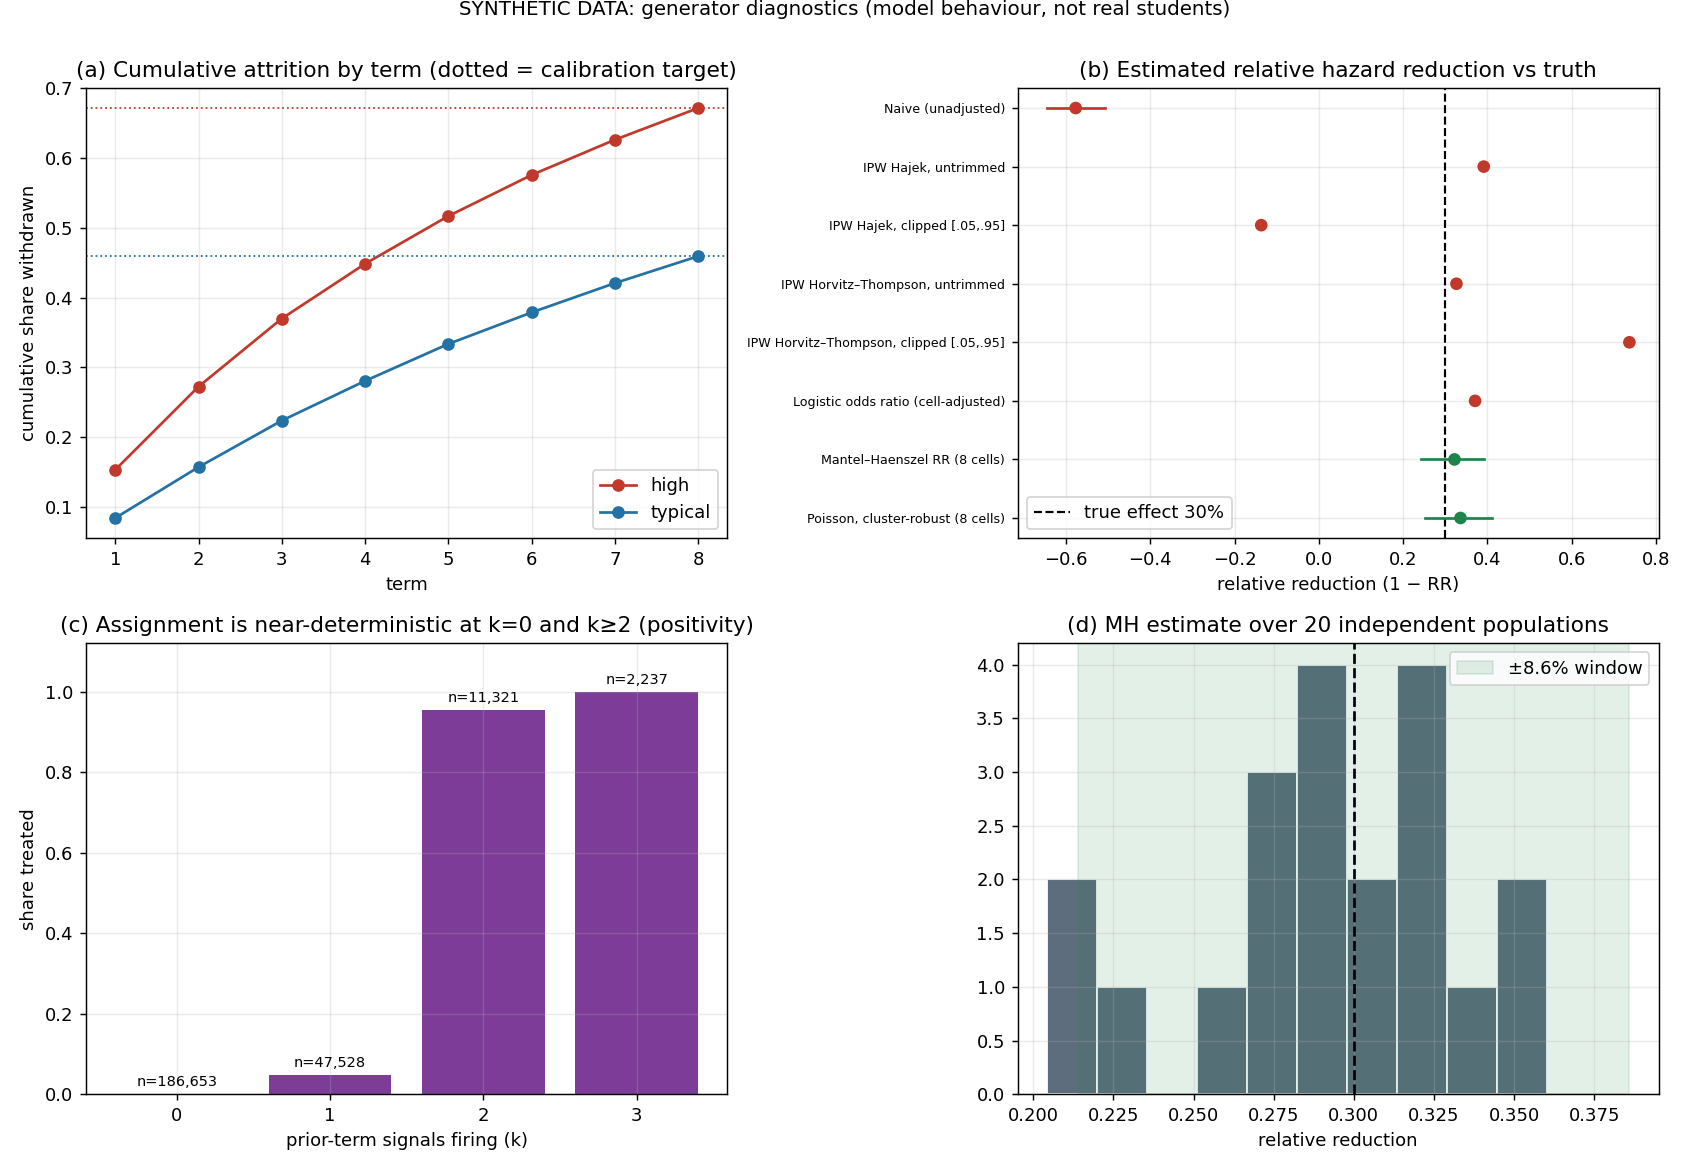
\includegraphics[width=5.2in]{../synthetic-data-generator/output/diagnostics.png}
\caption{Generator diagnostics (synthetic). (a) Cumulative attrition by term against the calibration targets. (b) Estimated relative hazard reduction by method against the true 30\%. (c) Assignment is near-deterministic when no signal or at least two signals fire. (d) The Mantel--Haenszel estimate over 20 independent populations.}
\label{fig:diag}
\end{figure}

\pfield{Skills demonstrated}
Simulation engineering in Python (numpy, pandas, SciPy, statsmodels); calibration by nested root-finding; reproducibility practice (named random streams, common random numbers, content hashes, pinned versions); automated data validation; documenting assumptions and open limitations; privacy-aware dataset design.

% ---------------------------------------------------------------- D3
\subsection{Deliverable 3: The analytics and the deck}
\begin{deliverable}{Deliverable 3 \quad Analytics notebook and slide deck}
\small 85-cell notebook, executed HTML export, 19-page slide deck (17 slides and 2 backup) \,$\cdot$\, \gh{tree/main/results-and-discussion}{\texttt{results-and-discussion/}}
\end{deliverable}

\pfield{Problem / Context}
Deliverable 3 asks for analytics on the dataset. I wanted more than a tour of charts. Because I know the truth behind the data, I could ask whether the workflow a Student Success Analyst would normally follow reaches the right conclusion, and where it does not.

\pfield{My role and contributions}
\begin{itemize}[topsep=1pt,itemsep=2pt,parsep=0pt]
\item Wrote the analysis so that it sees only what an analyst would see. The hidden state is used only in labelled places, always to \emph{grade} a result.
\item Copied the generator engine unchanged into the notebook and proved the copy faithful: it regenerates all eight tables with matching hashes and recovers the recorded calibration.
\item Built the prediction work with a leakage guard (features from earlier terms only), student-grouped five-fold cross-validation with the same folds for every model, fixed hyperparameters, and two ceilings that show how much of dropout is predictable at all. I excluded the regional tier from the flagging model on ethical grounds, and an ablation shows it adds almost nothing (AUC 0.656 with it, 0.655 without).
\item Ran the causal analysis with several estimators over 20 independent populations, an adjustment-set ladder and weight diagnostics, using \citet{peters2017} and \citet{gelman2020ros} to justify what can and cannot be concluded.
\item Audited targeting (who is flagged, who is missed, what false flags cost) and ran a sensitivity grid of 11 scenarios, each recalibrated to the same tier targets.
\item Turned the results into eight recommendations, a log of the limitations (DF-1 to DF-9), and a 19-page Beamer deck whose figures I redrew at slide size.
\end{itemize}

\pfield{Output}
The \gh{blob/main/results-and-discussion/student-retention-analytics.ipynb}{analysis notebook}, an executed \gh{blob/main/results-and-discussion/student-retention-analytics.html}{HTML export}, and the \gh{blob/main/results-and-discussion/student-retention-results-slides.pdf}{slide deck} with its LaTeX source. Table~\ref{tab:d3} gives the headline answer to each question, and Figure~\ref{fig:gap} shows the central one.

\begin{table}[htbp]
\caption{What the analysis found (synthetic; properties of the generator, not of real students).}
\label{tab:d3}
\centering\small
\renewcommand{\arraystretch}{1.15}
\begin{tabular}{@{}>{\raggedright\arraybackslash}p{0.30\textwidth}>{\raggedright\arraybackslash}p{0.63\textwidth}@{}}
\toprule
\textbf{Question} & \textbf{Headline}\\
\midrule
Is the generator valid? & Seven of seven comparable scorecard rows re-derive identically from the CSV files.\\
Can dropout be predicted? & Out-of-fold AUC 0.655 for boosted trees against 0.567 for a signal-count rule. A predictor that knew every student's hidden vulnerability would reach 0.683. A further 19.4\% of dropouts happen in term 1, before any prior record exists.\\
Does a good predictor say whether support works? & No. Raw comparison: support appears to raise dropout by 58\%. Stratifying on the model's risk score: $+7.4\%$. Stratifying on the assignment signals: $+32.2\%$ against a true 30\%.\\
Does the programme work? & Mantel--Haenszel and Poisson recover about 30\% (SD about 4 points over 20 populations). Inverse-probability weighting ranges from $-47\%$ to $+72\%$.\\
Who is missed? & 63.7\% of dropout events fall in terms with a clean record and no support. A model-ranked list would avert about 18\% more dropouts than the actual rule at equal capacity.\\
Is it robust? & Across 11 recalibrated scenarios the Mantel--Haenszel estimate stays near 30\%.\\
\bottomrule
\end{tabular}
\end{table}

\begin{figure}[tbp]
\centering
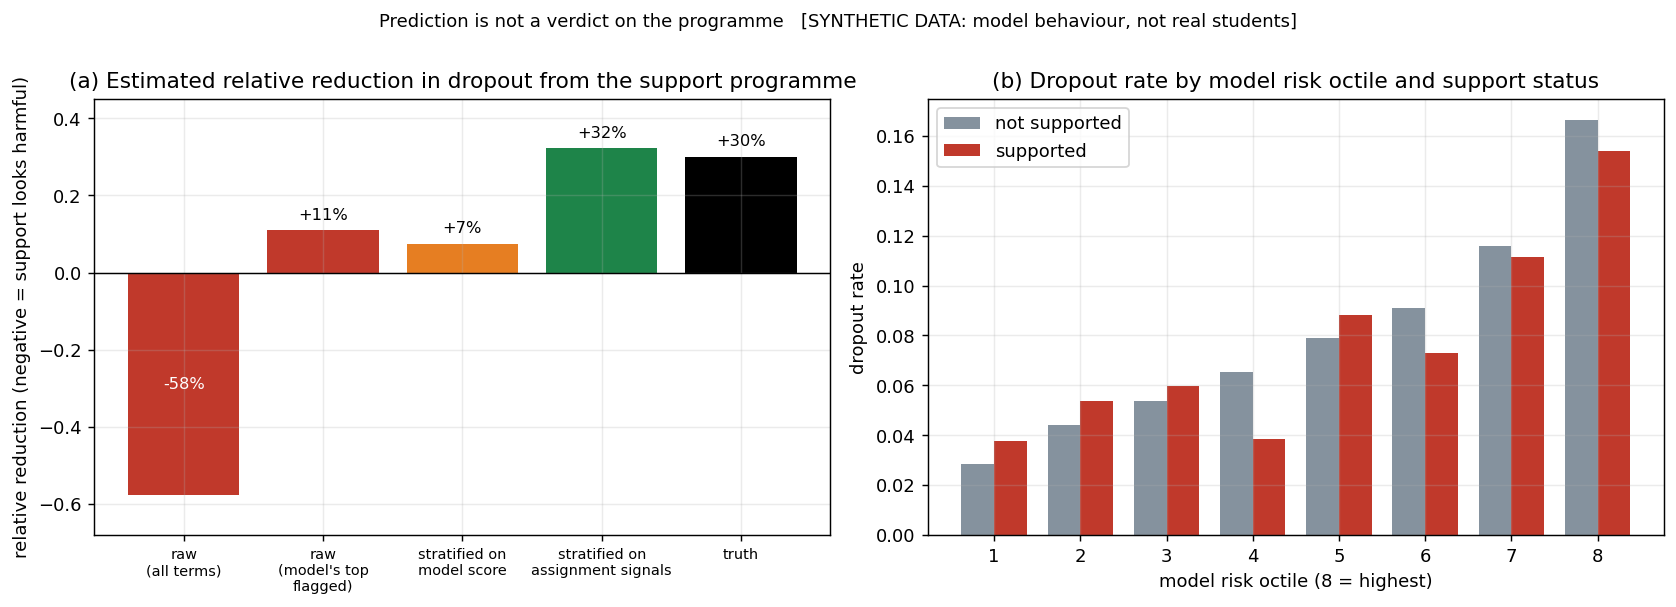
\includegraphics[width=6.0in]{../results-and-discussion/figures/fig3_actionability_gap.png}
\caption{The actionability gap (synthetic). (a) Five ways of estimating the programme's effect, against the true 30\%. (b) Dropout rate by model risk octile and support status.}
\label{fig:gap}
\end{figure}

\pfield{Skills demonstrated}
Applied causal inference and estimator diagnostics; predictive modelling with leakage control and honest evaluation \citep{james2013}; sensitivity analysis; reproducible notebooks; data storytelling for two audiences (a full notebook and a short deck); stating limits plainly.

% ============================================================ 4 REFLECTION
\FloatBarrier
\section{Reflection}
\label{sec:reflection}

\subsection{What did I learn?}
\begin{itemize}[topsep=1pt,itemsep=3pt,parsep=0pt]
\item \key{Matching a target is not validating a model.} Fitting two parameters to the tier rates shows only that the calibration loop converged. The checks with independent content are the correlation structure, the confounding check and the recoverability check, and I learned to report them separately.
\item \key{A good predictor is not a verdict on a programme.} The boosted model has a modest but real AUC of 0.655, yet stratifying on its own risk score gives $+7.4\%$ where the truth is 30\%. Knowing the assignment rule is what makes the comparison honest.
\item \key{Estimator choice can matter more than sample size.} With 50,000 students and the true propensity supplied, inverse-probability weighting still ranged from $-47\%$ to $+72\%$, because assignment is near-deterministic in some groups. Methods that borrow strength across groups had a standard deviation of about 4 points.
\item \key{An assumptions list is a design tool.} Having 51 parameters tagged \ptag{ASSUMED} turned into a ready-made agenda for sensitivity analysis.
\end{itemize}

\subsection{What challenged me?}
\begin{itemize}[topsep=1pt,itemsep=3pt,parsep=0pt]
\item \key{Results that did not match my own design.} The whitepaper states 70\% targeting precision and a 25\% false-flag rate; the generator realises about 16\% and 22\%. My scan showed that the pair is not jointly reachable under the chosen rule. The temptation was to tune the assignment parameters until the numbers matched. I held to the rule that a pre-specified quantity is not changed to make a check pass: I disclosed the difference, labelled it, and moved the question to the sensitivity analysis.
\item \key{A check that passes by a hair.} The held-out tier ratio sits at the upper edge of its band, so I labelled it ``pass (fragile)'' rather than ``pass''.
\item \key{Sources that disagree.} National attrition figures of roughly three and four in ten do not trace to the same cohort. Working out the provenance took real effort, and one reading (that a 29.4\% figure belongs to the Class of 2023) is still an inference from a table layout that I have flagged as open (OF-7).
\item \key{Keeping synthetic data from being mistaken for findings.} Every output carries a banner, individual-level tables carry no region names, and the recommendations end with a plain instruction not to act on these numbers.
\end{itemize}

\subsection{What am I proud of?}
\begin{itemize}[topsep=1pt,itemsep=3pt,parsep=0pt]
\item The project can be checked. A reader can regenerate all eight tables bit for bit, re-derive the scorecard from the CSV files, and see where each number came from.
\item The deliverables form one argument: the whitepaper states a model, the generator realises it, and the analysis tests what a standard workflow would conclude from its output.
\item The limitations are in the open. Twelve generator flags and nine analysis flags are logged with a status, including the ones that remain unresolved.
\item The analysis is written from an analyst's point of view and only then graded against the truth, which is the discipline I wanted a retention analyst to have.
\end{itemize}

\subsection{What would I improve?}
\begin{itemize}[topsep=1pt,itemsep=3pt,parsep=0pt]
\item \key{Bring the whitepaper in line with the generator.} Its targeting figures (Sec.~8 and Table~4) should describe the realised behaviour, the appendix should say that the near-determinism follows from the chosen parameters, the title page should carry a version line, and the pilot script that Appendix A mentions should either be added or the sentence reworded.
\item \key{Close the sourcing question} on the 29.4\% figure against CHED's underlying data, if it can be obtained (OF-7).
\item \key{Make the slide figures reproducible} by adding the script that draws them to the repository.
\item \key{Loosen the generator's simplifications.} The model has a single homogeneous effect, no carry-over from support into later grades, and no unmeasured assignment confounders, so the causal problem here is easier than a real one.
\end{itemize}

% ============================================================ 5 WHAT'S NEXT
\section{What Is Next}
\label{sec:next}

\subsection{Finishing this project}
The first thing I would do is publish a whitepaper v18 that fixes the inconsistencies listed above. After that I would resolve OF-7, add the figure script, and re-run the held-out check that the analysis did not repeat.

\subsection{Extending the science}
The analysis notebook already names the open questions:
\begin{itemize}[topsep=1pt,itemsep=2pt,parsep=0pt]
\item \textbf{Heterogeneous effects.} Allow the support effect to differ by student, which breaks the assumption that ranking by risk is optimal.
\item \textbf{The cost of building overlap into a rollout.} The analysis recommends a small randomised share of referrals so that every signal group has both treated and untreated students. I did not measure what that costs in support slots.
\item \textbf{The boosted model across scenarios.} The sensitivity grid recomputed the signal-count rule and the ceilings, but not the boosted model's accuracy (DF-5).
\item \textbf{Why stratifying on the model's score is biased.} I observed the bias but did not investigate its mechanism (DF-7, open).
\end{itemize}

\subsection{What real use would require}
Nothing in this repository should drive a decision about real students. A real programme would need permissioned administrative data, ethical review, and a head-to-head pilot of model-based allocation with a randomised share of referrals. That is the point at which the recommendations in Deliverable 3 stop being conclusions within a model and start being hypotheses.

\subsection{Where to find everything}
\begin{center}
\small
\renewcommand{\arraystretch}{1.15}
\begin{tabular}{@{}>{\raggedright\arraybackslash}p{0.30\textwidth}>{\raggedright\arraybackslash}p{0.62\textwidth}@{}}
\toprule
\textbf{Item} & \textbf{Location in the repository}\\
\midrule
Repository overview & \gh{blob/main/README.md}{\texttt{README.md}}\\
D1 whitepaper & \gh{blob/main/whitepaper/student-retention-data-generator-model.pdf}{\texttt{whitepaper/student-retention-data-generator-model.pdf}}\\
D2 generator and dataset & \gh{tree/main/synthetic-data-generator}{\texttt{synthetic-data-generator/}}\\
D3 notebook, HTML, slide deck & \gh{tree/main/results-and-discussion}{\texttt{results-and-discussion/}}\\
This portfolio & \gh{tree/main/culminating-activity}{\texttt{culminating-activity/}}\\
\bottomrule
\end{tabular}
\end{center}

\vspace{4pt}
\begin{tcolorbox}[colback=titlebox,colframe=titlebox,arc=3mm,boxrule=0pt,left=6mm,right=6mm,top=3mm,bottom=3mm]
\centering\sffamily\bfseries\color{paperblue}
This is the story of my work. The work is imperfect, the imperfections are documented, and all of it is visible.
\end{tcolorbox}

\bibliographystyle{plainnat}
\bibliography{references}

\end{document}
